\documentclass{article}
\usepackage[utf8]{inputenc}
\title{Empowering local IT with open-source tools}
\author{Lauri Võsandi}
\date{May 2015}
\usepackage{natbib}
\bibliographystyle{IEEEtranN}
\usepackage{graphicx}
\usepackage{url}
\usepackage{tikz}

\begin{document}

\maketitle

\section{Introduction}

Linux is an portable operating system kernel
\cite{linux-a-portable-operating-system} devised
by Linus Torvalds and it can be used in conjunction with other
userspace utilities such as GNU \cite{free-software-free-society} to build
a free and open-source operating system.
Cost to redevelop Linux kernel in traditional corporate setting
is estimated to be approximately \$ 1.4 billion
\cite{estimating-cost-of-linux-distro}, which is still a fraction
of the development cost of a whole distribution such as Ubuntu
\footnote{Ubuntu is an GNU/Linux distribution originally
designed for end users incorporating known applications such as Firefox and LibreOffice}.
Usual Linux distribution for desktop consists of thousands software packages
such as Mozilla, Firefox, LibreOffice, VLC etc.

Most of the packages are licensed under
GPL \cite{general-public-license} copyleft license or
more liberal licenses such as
MIT \cite{the-mit-license} and
BSD \cite{the-bsd-2-clause-license} \cite{the-bsd-3-clause-license}
which guarantee
three freedoms to the user:
a) right to get the source code of the software packages
b) right modify the programs and
c) right to redistribute the changes.
The controversial GPL license forces the changed versions
of the programs to remain under GPL license,
effectively forcing companies to release sources they
used to build commercial versions of the software.
In many occasions companies fail to follow the
rules  --
VMware was sued in Germany for failure to comply with GPL
\cite{vmware-sued} in March of 2015,
on the other hand Red Hat has been conducting
successful business using open-source for years.
In the past GPL has proven to be effective in court protecting
the interests of the authors or copyright holders to be precise.

Up to now Linux-based operating system deployment has been
error prone, time-consuming process and usually specific to
a particular distribution of Linux.
Linux-based operating systems have made significant
progress on the servers
\footnote{Google and Amazon have successfully used open-source software
and commodity hardware to build enterprise grade cloud}
and embeddeded systems
\footnote{Android is the market leader in smartphones and it is composed of open-source components such as Linux}, but
the workstations and laptops are lagging behind.
Linux-based operating systems also have a reputation
of being overly complex to set up for a novice computer user and
lacking native hardware support for certain vendors such
as Broadcom \cite{new-linux-broadcom-wi-fi-drivers-arrive} wireless chips and Nvidia
\cite{nvidia-seeks-peace-with-linux-pledges-help-on-open-source-driver}
graphics.
Even though there are now many laptop models available with
Ubuntu pre-installed, the marketing hype of
competitors outshines the struggles of open-source
operating systems on desktops and laptops.

%According to DistroWatch Ubuntu, ?? and ?? are the three most
%favored Linux distributions for end users.
In the major thesis technical solution to reduce
Linux-based operating system deployment time using
Btrfs filesystem is presented and in this paper the business aspects
of the solution and related services are discussed.


\section{Background}

Tiger Leap (Tiigrihüpe) was a program announced
by president Lennart Meri in 1996 with the plan to heavily invest
in computers and network infrastructure in Estonia.
As part of Tiger Leap program schools procured IBM PC-s and
other equipment.
As part of Look@World (Vaata Maailma) program
various web applications were unrolled for schools such as
eKool (e-school) in 2002 which is used to keep track of student attendance.
This transformed Estonia into an advanced paperless e-society.

It is common for software vendors to offer products for
educational institutions for sub-nominal prices or even for free
in order to gain userbase \cite{dreamspark} \cite{google-for-education}
\cite{apple-education-pricing}.
In the past Microsoft has offered it's products and
services at non-sustainable prices
for developing countries \cite{microsoft-giveaway}
Once the country has reached certain living standard the
pricing is adjusted accordingly.
As the users have been learning to use particular product,
reluctance to switch is increased due to training costs,
user fustration etc.
Andrew Lewis' quote \emph{'If you are not paying for it,
you're not the customer; you're the product being sold'}
\cite{user-driven-discontent}
illustrated by Geek \& Poke comic shown in
Figure~\ref{fig:free-model}
perfectly fits this scenario --
in a sense  teachers and schools are used by the companies
to market the products to children.


\begin{figure}[!htb]
\centering
\scalebox{0.6}{\includegraphics{images/pigs-talking-about-the-free-model.jpg}}
\caption{Free model illustrated by Geek \& Poke}
\label{fig:free-model}
\end{figure}





%Most often organizations submit to paying
%licensing fees at significantly higher prices due to increased
%user discontent because of switch.

Starting from the end of 2013 Microsoft does not consider Estonia a
developing country anymore. The implication of the change was that
the Microsoft Windows and Microsoft Office license fees would rise
from current 6 EUR to 60 EUR per month per machine.
According to Ernst and Young analysis Tallinn could save 490 000 EUR
within five years if they would give up Microsoft Office now.
Replacing Windows with Linux would save additional 210 000 EUR
\cite{ernst-young-report}.

This was the main motivation for Tallinn Education Department to try
out alternatives.
As change from Microsoft Office to LibreOffice was
certain, replacing operating system was more questionable and
more research was required.
In March of 2014 Tallinn Education Board decided
to pilot Linux in five educational sinstitutions:
Mustamäe Upper Secondary School,
Tallinn Mahtra Primary School,
Merivälja school,
Tallinn Mesimummu kindergarten and
Tallinn Tammetõru kindergarten in order
to determine potential problems and roadblocks.
In other words the pilot project was used to answer
the question \emph{can you take control over you IT infrastructure
with open-source?}

\section{Challenge}

This pilot project procurement bid was won by Arvuti Traumapunkt OÜ
\footnote{http://atrauma.ee} and
Silver Püvi hired author to take care of setting up infrastructure servers.
Most of the work so far has been done remotely in conjunction with
local IT-support.
Prior the project the author never had experience managing Linux based workstations.
The goal was to provide a platform which would be easier than current Windows
workstations.
In retrospective maintaining Linux-based and in fact
Windows workstations as well concerns several aspects:

\begin{itemize}
\item Provisioning - getting the initial software setup onto the computer
\item Updating - keeping the software up to date
\item Configuration management - adjusting configuration of various software components
\item Central authentication - keeping user accounts off the machines
\item Networked storage - keeping user files off the machines
\end{itemize}

The need for configuration management, central authentication
and networked storage was recognized immideately.
Puppet was chosen for configuration management due to it's
enterprise capabilities and vibrant community.
Foreman was used as Puppet web interface to provide
overview of the inventory as shown in Figure~\ref{fig:foreman}.
Initially Puppet was used to also perform software updates, but
it turned out to be a bad idea because even though Ubuntu package
management performs well for most cases, there are still some
corner cases which may render the whole package management
system unusable.

\begin{figure}[!htb]
\centering
\scalebox{0.5}{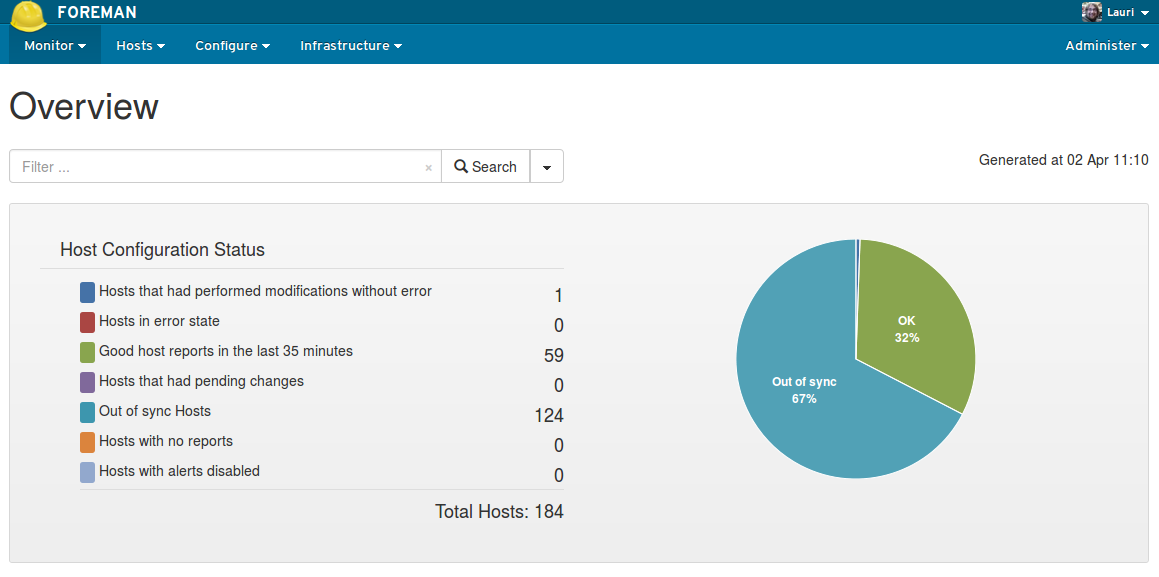
\includegraphics[scale=0.6]{images/foreman.png}}
\caption{Foreman}
\label{fig:foreman}
\end{figure}

Initially OpenLDAP was chosen for authentication and authorization,
but later we switched to Samba4 in order to provide better
interoperability with Windows workstations.
In fact Samba implements Microsoft Active Directory functionality
to large extent,
making it possible to avoid licensing fees while still maintaining
compatibility with Windows workstations.

\section{Roadblocks}

The project team was aware that there will be problems,
but many of the problems came unanticipated.

For example European Union mandates that all governmental documents to
be accessible in open formats, but at the same time
various European Union bodies distribute PDF forms which
embed forms using proprietary XFA format \cite{xfa}
and such PDF files are currently not
usable by any open-source tool, forcing the computer
user to fall back to Adobe Reader.
This problem was faced on several occasion while
carrying out the migration.
This is a classic example of vendor lock-in and
it could be avoided, especially in public sector.

Many computer users, especially of older generation
had grown accustomed to
Microsoft Office and found it frustrating
if certain functionality was exposed
via different menu structure.
Also some of the materials prepared on Microsoft Office,
fail to display properly due to proprietary fonts
bundled with Windows.
As Google faced similar issues on Google Chromebooks,
they've created substitute fonts which can also be installed
on Ubuntu machines \cite{substituting-fonts}.

Canon printers turned out to be troublesome to install
for Ubuntu as Canon distributes the drivers in a binary-only
format.
Instead making use of
Common Unix Printing System \cite{cups} they've
developed several independent printing stacks and
as of spring 2015
Canon CAPT driver tends to freeze \cite{capt}.
At the same time we didn't have any issues
with Hewlett Packard, Samsung or Lexmark printers.

Smarttech SB480 and SB600 smart whiteboards were also
troublesome to set up in the beginning.
While SB600 uses standards-compliant interfaces
to talk to the operating system without needing extra drivers,
SB480 is a highly customized piece of hardware that
needs additional drivers which are not available
out-of-the-box and Smarttech provided drivers
worked only on few occasions.

In addition to drivers the userspace application
Smart Notebook was outdated for Linux distributions --
version 11 was available for Ubuntu
while version 14 was already unrolled for Windows,
thus users were not happy about the downgrade.
The schools had procured smart whiteboards with
the assumption of having software upgrades for free,
but eventually Smarttech admitted that their business
model was no longer viable and they would start charging
license fee for Smart Notebook upgrades.

\section{Transforming experience into services}

\subsection{Ubuntu deployment service}

As part of the major thesis a more efficient way of deploying Linux-based
workstations was devised.
The resulting software components were used to build an service for
distributing Linux-based operating system templates which can be used to
quickly deploy workstations, laptops and netbooks customized
for particular purpose within 15 minutes over the Internet.
Currently we're maintaining template of Ubuntu 14.04 LTS based
workstation which uses lightweight MATE desktop as
shown in Figure~\ref{fig:mate}.

\begin{figure}[!htb]
\centering
\scalebox{0.5}{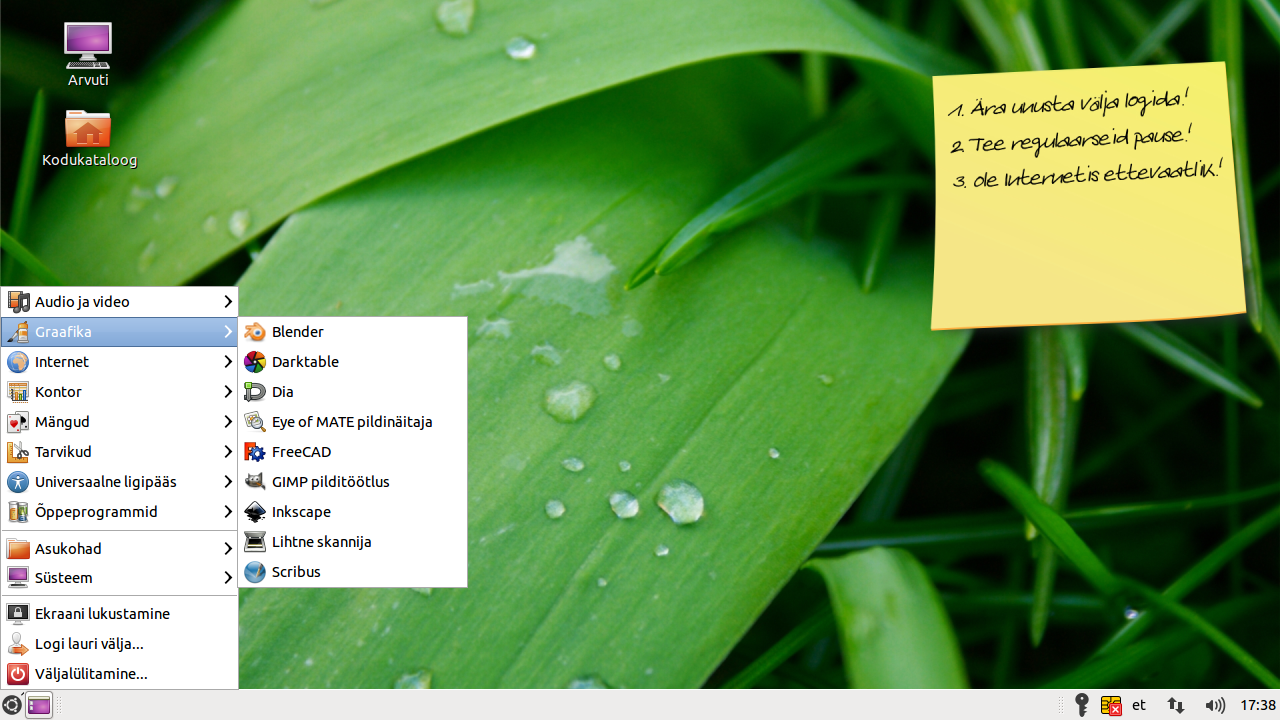
\includegraphics[scale=0.5]{images/edu-workstation}}
\caption{MATE desktop}
\label{fig:mate}
\end{figure}

We've fine-tuned MATE to slightly mimic Windows XP layout to provide
familiar looks to older generation of users.
The user interface and keyboard langauge is Estonian by default,
the template includes
Estonian ID-card software,
Mozilla Firefox, LibreOffice etc.
The innovative aspect of the solution was making commercial use of
emerging Btrfs filesystem and LXC container technologies.

\subsection{Software packages}

In addition to Ubuntu software repositories
we operate an APT repository of 3.6GB which contains
certain proprietary software components necessary
to ease the usage of various hardware equipment.
The repository also contains patched versions of
open-source software which have been modified to cater the
needs of the customers - for example
ID-card enabling packages for Linux based terminal-server,
which are used by National Library of Estonia.

\subsection{Remote management}

As the Ubuntu is being continuously improved it also requires
continuous maintenance of the templates provided by the service.
Maintaining a well oiled Linux based workstation
requires extensive knowledge of
how the Linux-based operating system is put together of
thousands of software components and how they interact with each other.
Occasionally skills to dive into C code are necessary
in order to resolve problems.

The templates we ship are automatically associated with
the Puppet master instance which lets us manage
the configuration of the machines and apply critical security updates.


\subsection{Identity service}

Our customized Ubuntu 14.04 template integrates
well with existing Active Directory deployments
and Windows file shares.
We also provide Active Directory compatible
authenticationa and authorization service
for Windows, Ubuntu and Mac OS X workstations using Samba4.
This service is mainly targeted towards
smaller organizations lacking local
infrastructure and manpower to operate such services,
but still wishing to take advantage of centralized
authentication.

\subsection{ownCloud}

ownCloud shown in Figure~\ref{fig:owncloud}.
is an open-source project which implements
Dropbox functionality to large extent.
Unlike Dropbox, ownCloud can be deployed
on company's or trusted service provider's servers
seamlessly integrating with existing infrastructure
\cite{deploying-owncloud}.
The ownCloud business model is built around selling
enterprise version of ownCloud which has more features
such as Shibboleth authentication which is used by universities
\cite{owncloud-closes-2.5-million-usd}.
There are synchronization clients available
Ubuntu, Windows, Mac OS X, Android and iPhone
making it possible to easily share photos and documents within
an organization.

\begin{figure}[!htb]
\centering
\scalebox{0.5}{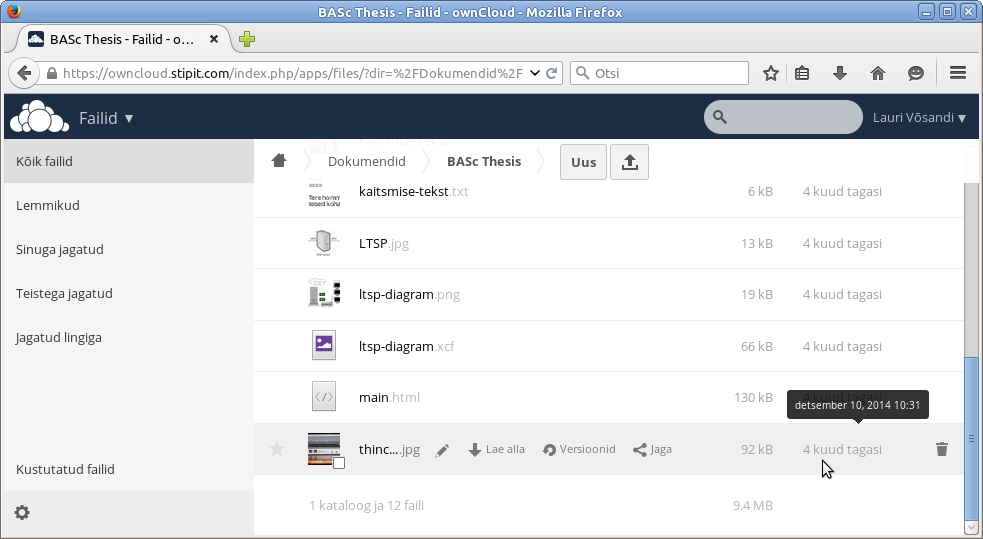
\includegraphics[scale=0.5]{images/owncloud}}
\caption{ownCloud web interface}
\label{fig:owncloud}
\end{figure}

For major customers we provide installation,
configuration and maintenance of on-site ownCloud instance.
We also provide shared ownCloud instance
for our customers which is configured to work
in conjunction with our authentication service.
We're planning to add single-sign on
for all the workstations joined to our domain.

Even though ownCloud is one step towards the right direction
there is still long way to go.
Eventually we would like to see more standardization
in the cloud sector, making it possible
to share documents between ownCloud instances,
Google Drive, Microsoft OneDrive, Dropbox etc.

\subsection{Training}

As of January 2015 the author has acquired both:
LPIC-1: Linux Server Professional Certification \cite{lpic-1} and
LPIC-2: Linux Network Professional Certification \cite{lpic-2},
making it easy to conduct Linux related trainings.
In co-operation with Estonian IT College we're providing
following courses based on exclusively open-source tools
about firewalling, virtual private networks
\cite{firewalls-and-virtual-private-networks};
authorization and authentication \cite{authentication-and-authorization}.
In addition to those we've worked directly with companies to
provide know-how about what they need:
Linux containers using LXC;
hardware virtualization with KVM;
Postgres administration;
Python programming etc.


\section{Summary}

The pilot project carried out by Tallinn Education Department
served it's goal to identify the barriers for open-source adoption.
Complete migration from Windows to Linux is not planned in the
near future, but the Tallinn Education Department confirmed
their decision to stick with LibreOffice and
support dual-boot scenarios for future deployments.
For example the tender documents published by
Tallinn Education Deprartment for rental of
2300 desktops and 1600 laptops for schools
\cite{arvutite-rentimine-koolidele} and
850 desktops for kindergardens
\cite{arvutite-rentimine-lasteaedadele}
specify that the machines have to support
Ubuntu 14.04 or later long-term support version out-of-the box
without installing additional drivers.
We're working with Tallinn Education Department
to bring customized and up to date Linux desktop experience
to the rental machines as well.

The warmest reception of Ubuntu and LibreOffice
was met at one of the kindergardens where the computers were
introduced as part of the project.
Also the younger generation was able to handle
different environment much better,
probably due to the fact that smartphones
are already very different and for them Ubuntu
is just yet another slightly different user interface.
Thus we recommend switching operating systems
where the change is imminent -
for example when computers are upgraded or introduced in the
first place.

As a side effect we discovered that schools were in fact
using outdated workflows, such as composing documents using
generic word processor and printing the documents.
The long term solution would be to use web-based
workflow-specific applications (in contrast
to generic word processing).
According to the
information society development plan
\cite{eesti-infouhiskonna-arengukava} published by
Ministry of Econimic Affairs and Communications
there will be heavy investments to Internet access across Estonia.
According to the plan Estonia should have 95\% of
it's communications done in a paperless manner by 2020 and
even more importantly all bills should be sent in
electronic machine-readable format.
Additionally HITSA (Information and Technology Foundation for Education)
is updating the ways computers are used in the education
and major component of that is the webification of
learning materials, thus future procuments require
teachers and proffessors to publish documents that
use open standards such as web instead of relying on
proprietary technologies such as Adobe Flash or
Windows-only binaries paving way to BYOD
\footnote{Bring Your Own Device generally means that instead of
organization provided device the employee is using her own
equipment to work}.


%Thus we highly reccommend for
%developing countries to learn from the experience of Baltic countries
%and avoid vendor lock-in by building IT infrastructure using
%open-source components in the first place
%rather than licensing proprietary components
%at non-sustainable prices.
%Even if it's not possible in all scenarios to rely 100\% on open
%solutions, it is necessary to understand the business
%model of the companies that are providing the products and services
%and whether the model is sustainable in long run.

The author used the experience gained in the Tallinn migration project
to bootstrap Ubuntu deployment, remote management,
software packaging and ownCloud services.
Software packaging services, Puppet remote management
and earlier version of identity services
are already unrolled to our customers.
Deployment, ownCloud and Samba4 based identity services are in final testing phase.
We have customers popping up in other market segments such as defence and health care.
We will also continue providing open-source consulting.
Additionally we are co-operating with various e-service providers
such as e-kindergarden to provide up-to-date
Ubuntu OS foundation to consume their web based services.
Thus is a way we're contributing to the advancement of
standards-compliant web services and innovative usecases
for both public and private sector as standards-compliant
web and multi-platform applications are the enabling factor for
BYOD.


\section{Conclusions}

There are various political, economic, societal reasons why
companies and governments wish to use open-source software.
Open-source components significantly decrease time to market
as products can be quickly prototyped and delivered using
readily available components without spending time or finances on
software component producement, licensing or outsourcing.
%Nearly all start-ups rely on readily usable open-source
%components and modern start-up scene would not be the same
%without open-source.
Open-source development model cuts costs and due to
it's deduplicative nature enables pooling of resources
in order to have better service or product in long run
for all the participants.

In addition to financial aspects, the privacy concerns rised by
Edward Snowden in 2011
\cite{edward-snowden-revelations}
has pushed various governments to seek for alternatives
to relying on proprietary technology.
For example
European Union has recognized the need to fund open-source projects
mainly due to privacy and security concerns.
\cite{eu-should-finance-open-source}.
Similariliy Indian Government mandates use of open-source technologies
in order to reduce total cost of ownership and to ensure
strategic control of e-Governance applications and systems
\cite{open-source-adoption-at-government-of-india}.

Apple's entrance to the mainstream computing market
also had significant impact on the industry,
occasionally in favour of open-source community --
for example Apple's decision to not support
proprietary Adobe Flash technology on iPhone
\cite{apple-pretty-much-murdered-mobile-flash}
has paved way for adaption of open solutions such as HTML5.
Even Microsoft is changing and adapting to changing markets,
for example Microsoft launched .NET distribution for
Linux and Mac in the end of April 2015
\cite{microsoft-launches-net-distribution-for-linux}.
The companies are starting to see
software as expense instead of competitive advantage
\cite{eesti-telekom-annab-arisektorile-suunatud-tarkvara-vabakasutusse}.
In certain IT industry sectors the open-source
development model is already becoming the dominant design.

Open-source can be seen as enabling factor for creation of jobs.
Political decisions that foster open-source communities and businesses
also bring increased employment in these sectors,
so cash flow that otherwise would be allocated for
license expenditures
are invested back into local workforce
pushing the knowledge based society and economics further ahead.
To answer the question -- \emph{Yes, open-source can be used
to take control over your IT, but it takes time, patience and
careful long-term planning}.

%Western world and especially countries of post-soviet syndrome
%have difficulties fully grasping the whole topic and there's
%a lot of misconceptions about open-source and Free Software,
%thus awareness raising is necessary.
%Estonian Free and Open-Source Software Association
%\footnote{\url{http://alvatal.ee/en/}}
%is the corresponding body in Estonia and we have a lot of work to do.



\appendix

\clearpage

\bibliographystyle{plain}
\bibliography{references}


\end{document}
